\FloatBarrier
\chapter{Tabellen en grafieken}
\label{sec:Tabellen en grafieken}

\makeatletter
\setlength{\@fptop}{0pt}
\makeatother
\captionsetup{justification=justified,singlelinecheck=false}

\captionof{table}{Verliesco\"effici\"ent bij stroming door een cirkelvormige bocht van 90\deg}
\begin{tabular}[t]{p{12cm} p{5cm}}
	\vtop{\null\hbox{
		\begin{tabular}{l c c c c c}
			$r/D$        & 1    & 2    & 4    & 6    & 10   \\
			\hline
			$\zeta$ glad & 0.21 & 0.14 & 0.11 & 0.09 & 0.11 \\
			$\zeta$ ruw  & 0.51 & 0.30 & 0.23 & 0.18 & 0.20 \\
		\end{tabular}
	}}
	&
	\vtop{\null\hbox{
		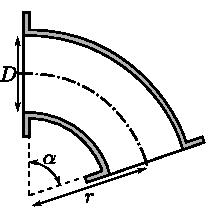
\includegraphics{fig/appendix/Bocht}
	}}
\end{tabular}
\captionof{table}{Correctiefactor voor cirkelvormige bochten met andere hoeken}
\begin{tabular}[t]{p{12cm} p{5cm}}
	\vtop{\null\hbox{
		\begin{tabular}{l c c c c c c}
			$\alpha$ & 30\deg & 60\deg & 90\deg & 120\deg & 150\deg & 180\deg   \\ 
			\hline
			$k$    & 0.4    & 0.7    & 1      & 1.25    & 1.5     & 1.7 \\
		\end{tabular}
	}}
	&
\end{tabular}
\captionof{table}{Correctiefactor voor geleidelijke verwijding}
\begin{tabular}[t]{p{12cm} p{5cm}}
	\vtop{\null\hbox{
		\begin{tabular}{l c c c c c c c c c c}
			$\alpha$ & 6\deg & 10\deg & 15\deg & 20\deg & 30\deg & 40\deg & 50\deg & 60\deg & 70\deg & 90\deg \\ 
			\hline
			$k$    & 0.14    & 0.20    & 0.30      & 0.40    & 0.70     & 0.90 & 1.00 & 1.10 & 1.10 & 1.00 \\
		\end{tabular}
	}}
	&
	\vtop{\null\hbox{
		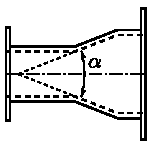
\includegraphics{fig/appendix/Verwijding}
	}}
\end{tabular}
\captionof{table}{Verliesco\"effici\"ent bij stroming door een plotse vernauwing}
\begin{tabular}[t]{p{12cm} p{5cm}}
	\vtop{\null\hbox{
		\begin{tabular}{l c c c c c c c c c}
			$D_1/D_2$ & 4.0 & 3.5 & 3.0 & 2.5 & 2.0 & 1.5 & 1.3 & 1.1 & 1.0   \\ 
			\hline
			$\zeta$    & 0.45    & 0.43    & 0.42      & 0.40    & 0.37     & 0.28 & 0.20 & 0.01 & 0 \\
		\end{tabular}
	}}
	&
	\vtop{\null\hbox{
		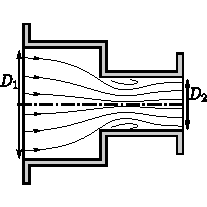
\includegraphics{fig/appendix/Vernauwing}
	}}
\end{tabular}
\begin{figure}[ht]
	\caption{Moody diagram}
	\label{fig:Moody diagram}
	\centering
	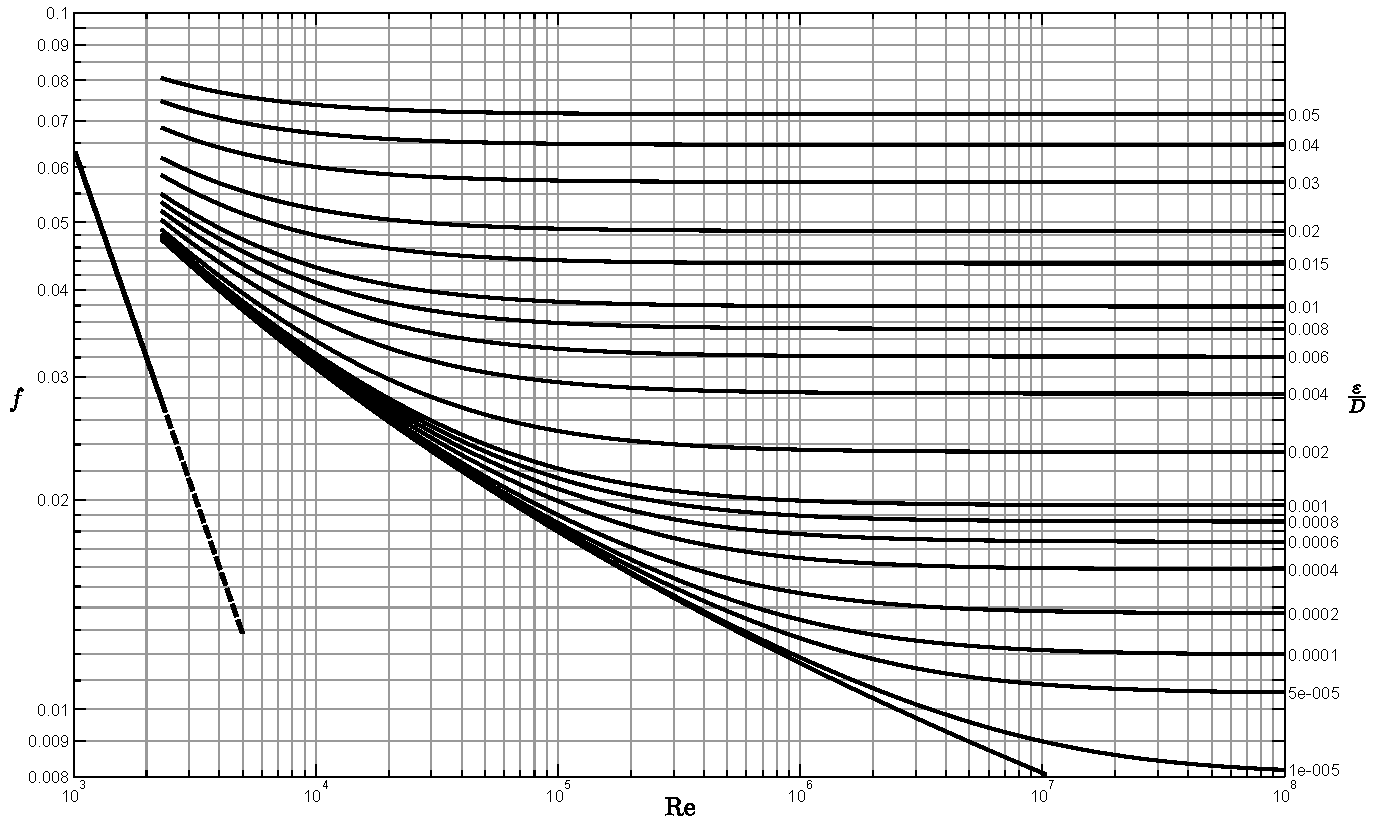
\includegraphics[width=22cm, angle=270]{Moody_diagram.pdf}
\end{figure}